\htwo{Service Worker}

\hthree{Allgemeines}

Web-Worker sind JavaScript-Skripte, die als Background-Task ausgeführt werden. Sie können zum Beispiel dazu verwendet werden, um eine Webseite offlinefähig zu machen oder Push-Notifications zu implementieren.  Um einen Web-Worker zu starten, ist es empfehlenswert zu prüfen, ob der Browser Web-Worker unterstützt.

\hfour{Life Cycle Events} 

Ein Service Worker hat verschiedene Events: 

\hfive{"Install event"}

Das Install-Event wird getriggert, nachdem der Service Worker registriert wurde. Dort werden normalerweise die Abhängigkeiten installiert. Z.B.: der statische Cache wird dort gefüllt 

\hfive{"Activated event"}

Bei der Erstinstallation wird das Activated Event unmittelbar nach der Installation ausgelöst. Wenn es einen neuen Service Worker für dieselbe Seite gibt, wird dieser nur installiert. Die Aktivierung erfolgt jedoch erst in der nächsten Sitzung. Das Activated Event wird in der Regel dazu verwendet, alte Ressourcen aufzuräumen. Z.B.: die Caches des vorherigen Service Workers werden geleert

\hfive{"Fetch event"}

Das "fetch"-Event wird jedes Mal aufgerufen, wenn eine Ressource des Servers angefordert wird. Es fängt diese Anfrage ab, um zum Beispiel mit den Daten aus dem Cache zu antworten.

\hfive{"Push event"}

Das Push Event wird getriggert, wenn der Server ein Push Event sendet, auf das der Client "subscribed" hat.

\begin{figure}[h]
    \centering
    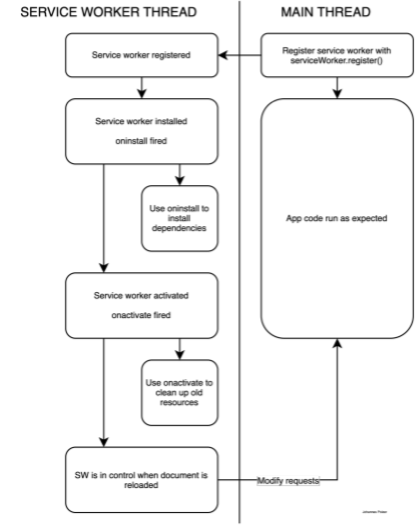
\includegraphics{media/ServiceWorker/lifecycle.png}
    \caption{Service Worker Lifecycle}
    \cite{MDNCacheAPI}
\end{figure}

\hfour{Registrierung eines Service Workers}

Ein Service Worker kann über das "serviceWorker" Objekt des "navigator" Objekts registriert werden. Da Service Worker nicht in allen Browsern unterstützt werden, muss davor überprüft werden, ob der Browser ein Service Worker unterstützt, um Fehler zu vermeiden.

\typescript{code/ServiceWorker/register.ts}{Registrieren eines Service Workers}
\pagebreak
\hthree{Implementierung eines Caches}
Der folgende Code zeigt, wie ein Service Worker mit der Cache-API zur Verwendung eines statischen und dynamischen Cache programmiert wird:

\typescript{code/ServiceWorker/cache.ts}{Verwendung der Cache-API in einem Service Worker}
